\documentclass[../main.tex]{subfiles}

\begin{document}
    
\subsubsection*{Methodology}
\subsubsection*{Data analysis}

Figure \ref{fig:4-Laserleistung-Resonatorlaenge} shows the laser output power plottet against the length of the resonator (measured from the left laser holder to the right laser holder). A linear fit of the shape $P(L) = \alpha\cdot (L - L_{th})$ was chosen as a rough estimate for the threshold length $L_{th}$ for lasing.

\begin{figure}[H]
    \centering
    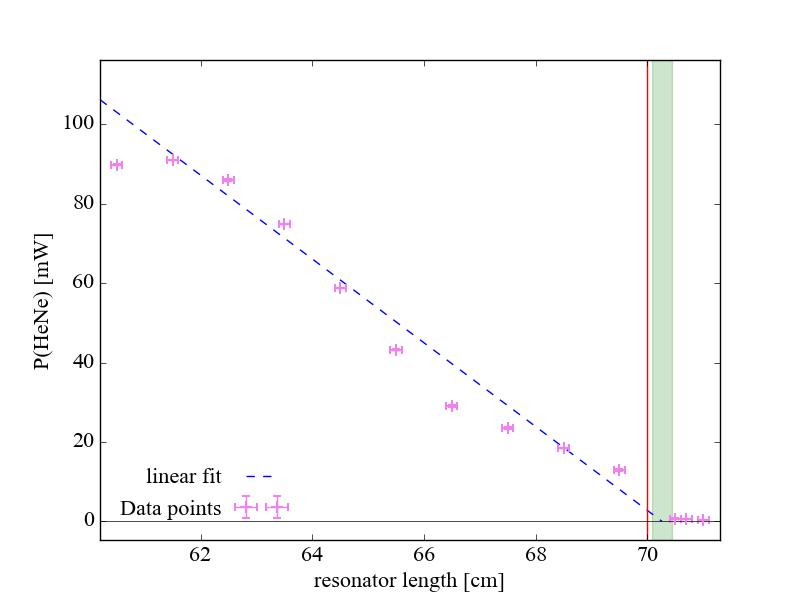
\includegraphics[width = 11cm]{Bilddateien/4-Laserleistung-Resonatorlaenge.jpg}
    \caption{Dependance of laser power from resonator length. The red vertical line represents the theoretical maximum resonator length $\color{red}{\SI{70}{\cm}}$, where lasing still occours. Its experimental counterpart $\color{ForestGreen}{L_{th} = \SI{70.26(18)}{\cm}}$  is colored green.}
    \label{fig:4-Laserleistung-Resonatorlaenge}
\end{figure}

\noindent Even though the theoretical and experimental values for the threshold length are within $\SI{3}{\mm}$ error range of eachother, according to their uncertainties they are not comptatible. 

\end{document}